\documentclass[11pt,letterpaper]{article}

\usepackage{graphicx}
\usepackage[margin=0.90in]{geometry}
\usepackage[T1]{fontenc}
\usepackage[utf8]{inputenc}
\usepackage{authblk}
\usepackage{fancyhdr}
\usepackage{lastpage}
\usepackage[parfill]{parskip}
\usepackage{subcaption}

\pagestyle{fancyplain}
\fancyhf{}
\fancyfoot[R]{\footnotesize Page \thepage\ of \pageref{LastPage}}

\renewcommand{\headrulewidth}{0.0pt} % No header rule
\renewcommand{\footrulewidth}{0.4pt} % Thin footer rule

\begin{document}

\title{Virtual Actor Space for On Demand Distributed Computation}
\author[1]{Benjamin Bengfort}
\author[2]{Allen Leis}
\author[1]{Konstantinos Xirogiannopoulos}
\affil[ ]{Department of Computer Science}
\affil[ ]{University of Maryland}
\affil[1]{\textit{\{bengfort,kostasx\}@cs.umd.edu}}
\affil[2]{\textit{aleis@umd.edu}}

\date{October 21, 2015}

\maketitle
\section*{Introduction}

\begin{figure}[h]
	\centering
    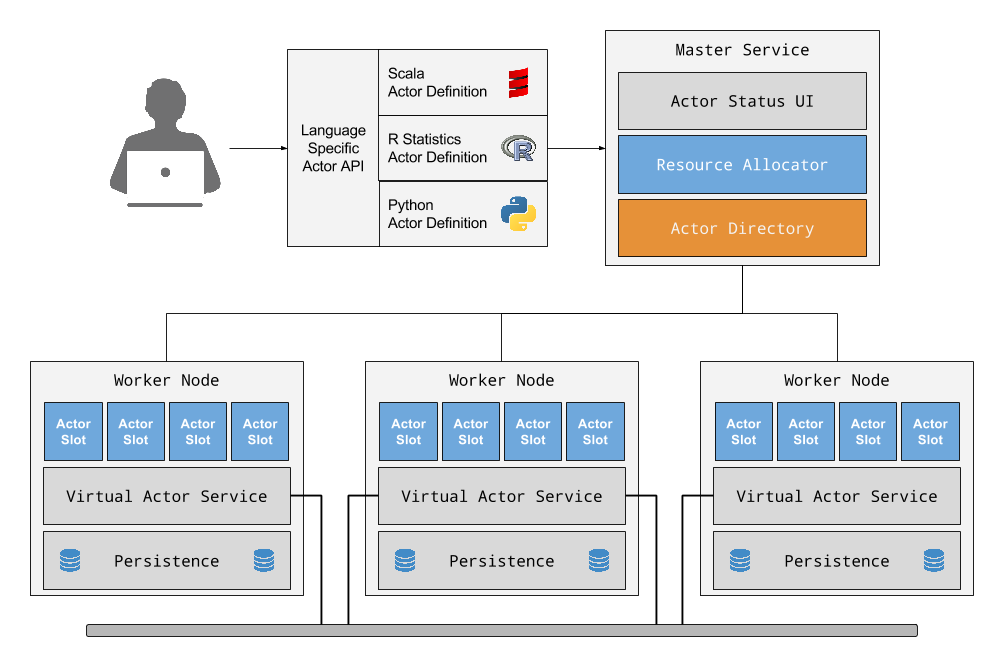
\includegraphics[width=0.8\textwidth]{figures/architecture.png}
    \caption{\textsf{Proposed architecture of a virtual actor space that generalizes distributed computation in an on demand fashion. A master node controls job submission and resource allocation, while worker nodes instantiate Actors in actor slots.}}
    \label{fig:performance}
\end{figure}

\bibliographystyle{plain}
\bibliography{papers}

\end{document}
